% Figure: the learned encoder. Rendered by render_tables.py via render_figures.encoder_forest from the run files of the
% two studies of the learned encoder; nothing numeric is typed here.
% supplement-ref supp:learned-swap=S6.4
% supplement-ref supp:learned-development=S6.2
\begin{figure}[!htbp]
\centering
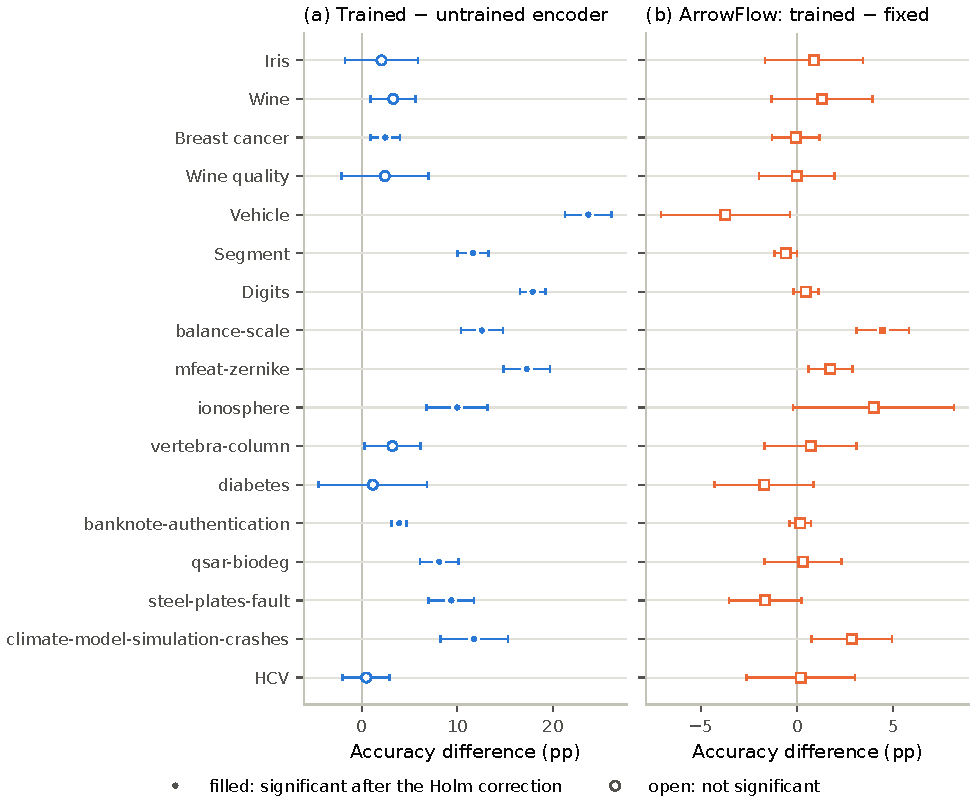
\includegraphics[width=0.92\textwidth]{figures/data/fig9_learned_encoder.pdf}
\caption{\textbf{Can the ranking signal train the encoder?} Accuracy differences, in percentage points, with 95\% intervals (not simultaneous); positive favors the trained encoder. The two panels have different scales. The intervals are not adjusted for multiple comparisons, so an open mark's interval can exclude zero. (a)~The classifier of Section~\ref{sec:learned-encoder}, an encoder network and one ranking layer of class filters, with the encoder trained by the converted motions, minus the same classifier with the encoder left at its random start. At that start, the weights of the encoder's first two layers are drawn uniformly from 0 to 1. Training lowers the mean error over the datasets from 25.5 to 17.2 percent. (b)~ArrowFlow with each view's fixed encoder replaced by the trained encoder network, minus ArrowFlow with its fixed encoder. For every split, both use the configuration that ArrowFlow's own tuning chose on the inner folds of that split's training partition. The swap also drops the polynomial expansion and the projection strategies (Section~S6.4). The mean error falls from 15.5 to 14.9 percent. Marks are circles in panel~(a) and squares in panel~(b). Filled marks remain significant after a Holm correction across the seventeen datasets: 11 in panel~(a) and 1 in panel~(b). The trained encoder has the higher mean accuracy on all 17 datasets in panel~(a) and on 11 of the 17 in panel~(b). The target conversion was developed on twelve of these datasets, all but Wine quality, banknote-authentication, qsar-biodeg, climate-model-simulation-crashes and HCV (Section~S6.2). HCV: hepatitis C virus.}
\label{fig:learned}
\end{figure}
